\documentclass[twoside,11pt,ShortChapTitles]{BYUTextbook}

\usepackage{soul}
\renewcommand{\vec}[1]{\ensuremath{\mathbf{#1}}}
\usepackage{siunitx}
\sisetup{round-mode = figures,
  round-precision = 3, scientific-notation=true}
  \usepackage{marginfix}

\usepackage{mathtools}






\setcounter{chapter}{7}

\begin{document}

\chapter{Numerical modeling of a Mass-Spring System}

In our last lab we started using Euler's method to solve physics problems.
We started with a problem we could do algebraically (a ball toss with no air
resistance), but then considered a problem that we could not do with just
algebra (a ball toss with air resistance). We did this by using the coupled
equations 
\begin{eqnarray*}
x(t+\Delta t) &=&x(t)+v(t)\Delta t \\
v(t+\Delta t) &=&v(t)+a\left( t\right) \Delta t
\end{eqnarray*}%
where for the first case 
\[
a\left( t\right) =-g 
\]%
and for the second 
\[
a\left( t\right) =-g+\frac{D\rho Av(t)^{2}}{2m} 
\]%
We said that to take on different problems using Euler's method, we only
have to change the acceleration term. And we can see that this was true for
our moving ball cases. We are going to take on a very different physical
system today, and we will see that even though it is very different, we can
still use Euler's method to describe the motion, and all we have to do is to
change the acceleration term again.

\subsection{Mass Spring Systems}

Let's review Hook's law for springs. Consider a system consisting of a mass
attached to a spring lying on a frictionless surface, as depicted in next
figure.\sidenote{%
A mass-spring system is often called a harmonic oscillator, it will show up
under this name in your PH121 book.}

\bigskip

\begin{center}
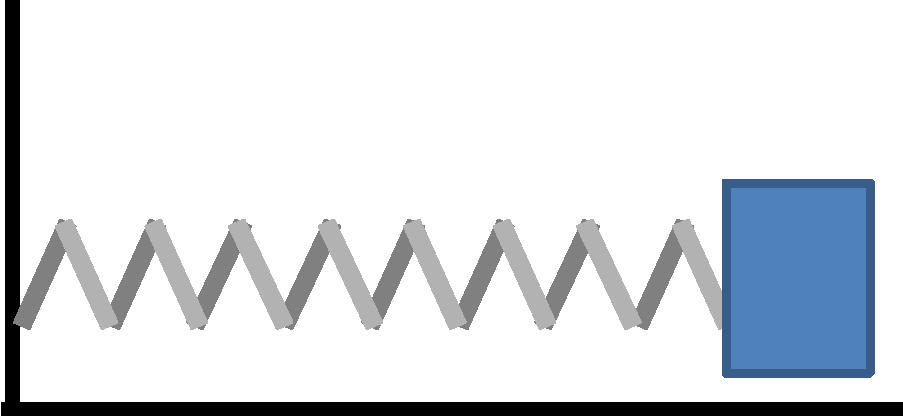
\includegraphics[width=0.8\textwidth]{Lab8_figs/mass_on_spring.pdf}
\end{center}

We assume that the spring strictly obeys Hook's law, $F=-kx$, where $k$ is
the spring constant and $x$ is the displacement from the equilibrium
position and $F$ is the spring force. There are only four inputs to this
system: the spring constant, the mass, and the initial velocity and initial
displacement of the mass. We turn to Newton's second law again to find the
acceleration. There is only one horizontal force.

\[
\Sigma F_{x}=ma=-kx 
\]%
so%
\[
a=-\frac{k}{m}x 
\]%
so we can write a set of coupled equations for the mass-spring system%
\begin{eqnarray*}
x(t+\Delta t) &=&x(t)+v(t)\Delta t \\
v(t+\Delta t) &=&v(t)+-\frac{k}{m}x(t)\Delta t
\end{eqnarray*}%
This is our Euler's method solution. We can use the same code as we started
with last lab for our one dimensional ball motion, but change the
acceleration to $a=-\frac{k}{m}x.$

\section{The exact mass-spring solution}

Of course, if you have taken PH123 you know we can also find an exact
solution for the motion of a mass-spring system's motion. Let's introduce or
review this here. It has quite a bit of calculus, so if you are concurrently
taking M12, don't worry. all you need is the answer at the end.

Given the simplicity of this system, it is fairly easy to write down an
equation that describes the motion. If your calculus skills are up to it, we
can rewrite this using differentials. Recognizing that acceleration is the
second time derivative of position, 
\[
a=\frac{dv}{dt}=\frac{d}{dt}\left( \frac{dx}{dt}\right) =\frac{d^{2}x}{dt^{2}%
} 
\]%
we can rewrite our spring acceleration as 
\[
\frac{d^{2}x}{dt^{2}}=-\frac{k}{m}x 
\]%
We call this type of equation a \emph{differential equation}. In our case,
we have an equation that involves a quantity, $x$, along with it's second
derivative. Because we have the second derivative of $x,$ it is called a
second order ordinary differential equation. If you stare at this equation
long enough, the solution becomes somewhat apparent. Ask yourself: for what
function can I take a derivative of twice and get the same function back
along with a negative sign and a constant? If you are far enough in your
M112 class the answer is obvious, a sine or a cosine.\sidenote{%
But if you are not far along in M112, don't worry. I am just trying to
motivate the calculus savvy reader to believe the position as a function of
time will be a sine or cosine function.} Of course it could also be a
combination of sines and cosines, so we can write a general solution 
\[
x(t)=a\sin \left( \omega t\right) +b\cos \left( \omega t\right) 
\]%
where $A$ and $B$ are constants and either could be zero. If we substitute
this in for $x$ in our differential equation, and take a couple of quick
derivatives we will see that our solution works so long as 
\[
\omega =\sqrt{\frac{k}{m}} 
\]%
Note that there are two undetermined constants in this expression, namely $a$
and $b$. Using a little trig\sidenote{%
OK, a lot of trig.}, we can rewrite this in an equivalent way\sidenote{%
This is where you should start paying attention if you are concurrently
taking M112.} 
\[
x(t)=A\sin \left( \sqrt{\frac{k}{m}}t+\phi \right) 
\]%
with the undetermined constants $A$, which represents the amplitude or
maximum displacement of the oscillation, and $\phi $ which is referred to as
a phase angle. This is true because the sum of a sine and a cosine function
is another sinusoidal function (think of all those trig identities you
memorized in your trig class!).

If we know what the initial displacement and velocity are, it is easy enough
to determine the values of $A$ and $\phi $. Doing so at this point would
distract from our discussion, so we will forgo the exercise for now. In any
event, the solution is oscillatory, as you would expect from a mass on a
spring.

\section{Adding friction (damping)}

A frictionless mass-spring system is obviously not too realistic. Many
oscillating systems will not fit our exact equation too well. Real masses
have frictional forces acting on them. A mass spring that experiences
friction is said to be \emph{damped}.

To modify our Euler code to use damping, we go back to Newton's second law
one more time. We need a new expression for the acceleration. There are two
forces that act on the spring: the spring force $F=-kx$\ which acts opposite
the displacement and a damping force $F=-bv$\ that acts opposite the
velocity. Here $b$ is the damping coefficient and is constant for a given
situation.

The dynamic equation that describes the system is then 
\[
\Sigma F_{x}=ma=-kx-bv 
\]%
We get a new acceleration 
\[
a=\frac{-kx-bv}{m} 
\]%
and use this in our coupled Euler equations.

\section{Review of the Euler Method}

Let's review how to turn this into an Euler solution.

Starting from the basic kinematic equation%
\[
\Delta x=v_{o}t+\frac{1}{2}at^{2} 
\]%
and assuming that for our time interval the change in velocity
(acceleration) is essentially zero, then 
\[
\Delta x=v_{o}\Delta t 
\]%
or%
\[
x_{f}=x_{i}+v_{o}\Delta t 
\]%
remember that we have only let our experiment run for a very small $\Delta t$%
, so even though it is accelerating, and the acceleration varies with $x$,
it would not have changed velocity much. And our equation will nearly work.
In the limit as $\Delta t\rightarrow 0$ our equation will be exact, just as
we said before.

Of course we want go an additional small time interval. That is, let the
experiment run from $t=\Delta t$ to $t=t+\Delta t.$ Then we can predict that
the next position will be 
\[
x(t+\Delta t)=x(t)+v(t)\Delta t 
\]%
As before we need to estimate a new velocity at the end of our time step, $%
\Delta t.$ We again use 
\[
v=v_{o}+at 
\]%
assuming a very small time interval (small enough that the acceleration does
not change a whole lot over the interval) I can write 
\[
v(t+\Delta t)=v(t)+a(t)\Delta t 
\]%
where I don't necessarily know that the acceleration is constant in time.
But just like in the last equation for position vs. time we did not assume
the velocity was constant (we just assumed it was essentially constant over
a small $\Delta t$) we will assume the acceleration is nearly constant over
the interval $\Delta t.$

We found (above) that for a frictionless mass-spring system Newton's second
law gave us 
\[
a=-\frac{k}{m}x 
\]%
This acceleration depends on position. It is not constant so technically we
can't use the kinematic equations. But it is constant enough over a very
small $\Delta t.$

Knowing the acceleration, we can use it in our velocity equation. 
\[
v(t+\Delta t)=v(t)-\frac{k}{m}x(t)\Delta t 
\]%
Now, we have two equations that project the position and speed forward in
time, based on what the position and speed currently are: 
\begin{eqnarray*}
x(t+\Delta t) &=&x(t)+v(t)\Delta t \\
v(t+\Delta t) &=&v(t)-\frac{k}{m}x(t)\Delta t
\end{eqnarray*}%
Just like before, these expressions are coupled: the new position depends on
the current velocity, and the new velocity depends on the current position.
To find the solution we will take a small step in time, $\Delta t,$ and
calculate a new position. We will also calculate a new speed. Then we will
use the new speed to find the next new position $\Delta t$ later, and the
new position to find another new speed. Once we step these two quantities
forward in time, we can repeat the process indefinitely.

In short hand these equations become%
\begin{eqnarray*}
x_{n+1} &=&x_{n}+v_{n}\Delta t \\
v_{n+1} &=&v_{n}-\frac{k}{m}x_{n}\Delta t
\end{eqnarray*}%
We have labeled each new $x$ and $v$ by how many time steps, $\Delta t$, we
have taken. The first $\Delta t$ will be $n=1,$ the second $n=2,$ and so on.
Just to be clear, let's again compare%
\begin{eqnarray*}
x(t+\Delta t) &=&x(t)+v(t)\Delta t \\
x_{n+1} &=&x_{n}+v_{n}\Delta t
\end{eqnarray*}%
This means that we start with the initial velocity, $v_{0}$ at the initial
position $x_{0}.$ We use these to calculate the position $x_{1}$ and the
speed $v_{1}$ a time $t=\Delta t$ later. Then we start with the initial
velocity, $v_{1}$ at the initial position $x_{1}$ and use the equations to
calculate the position $x_{2}$ and the speed $v_{2}$ an additional time $%
\Delta t$ later ($t=2\Delta t$). Then we use $x_{2}$ and $v_{2}$ to find $%
x_{3}$ and $v_{3}$ and so forth.

\section{General form for the mass-spring system}

We can write our coupled equations in our general form for Euler's method if
we want to. Here is how they would look.

Starting with the second order differential equation 
\[
\frac{d^{2}x}{dt^{2}}=-\frac{k}{m}x 
\]%
we write this as two coupled first order differential equations: 
\begin{eqnarray*}
\frac{dx}{dt} &=&v \\
\frac{dv}{dt} &=&-\frac{k}{m}x=a
\end{eqnarray*}%
To relate this to our general form, 
\begin{eqnarray*}
\frac{dx}{dt} &=&v(t)=f(x,v,t) \\
\frac{dv}{dt} &=&a(t)=-\frac{k}{m}x\left( t\right) =g(x,v,t)
\end{eqnarray*}%
We can write these for time $t_{n}$ as%
\begin{eqnarray*}
f(x_{n},v_{n},t_{n}) &=&v(t_{n}) \\
g(x_{n},v_{n},t_{n}) &=&-\frac{k}{m}x\left( t_{n}\right)
\end{eqnarray*}%
or more compactly,%
\begin{eqnarray*}
f(x_{n},v_{n},t_{n}) &=&v_{n} \\
g(x_{n},v_{n},t_{n}) &=&-\frac{k}{m}x_{n}
\end{eqnarray*}%
which gives us what we need to understand our general form%
\begin{eqnarray*}
x_{n+1} &=&x_{n}+(\Delta t)f(x_{n},v_{n},t_{n}) \\
v_{n+1} &=&v_{n}+(\Delta t)g(x_{n},v_{n},t_{n})
\end{eqnarray*}%
Of course this is really just 
\begin{eqnarray*}
x_{n+1} &=&x_{n}+(\Delta t)v_{n} \\
v_{n+1} &=&v_{n}+(\Delta t)\left( -\frac{k}{m}x_{n}\right)
\end{eqnarray*}%
for our specific case. But sometimes it is easier to write a general routine
and then provide $f(x_{n},y_{n},t_{n})$ and $g(x_{n},y_{n},t_{n})$ for our
specific case in a subroutine\sidenote{%
The terms \textquotedblleft routine\textquotedblright\ and \textquotedblleft
subroutine\textquotedblright\ will be familiar to the computer science
majors. For the rest of us they mean \textquotedblleft
program\textquotedblright\ and \textquotedblleft
sub-program\textquotedblright\ or in MatLab \textquotedblleft
script\textquotedblright\ and \textquotedblleft function.\textquotedblright}%
. This way the main routine can be easily used over and over and only the
subroutines need to be rewritten if we change specific cases.

\section{Harder oscillation systems}

There are problems worse than damping. After all, if you have taken PH 123
you know that we can find a solution even to the damped case that is a
single equation (but it is hard to do). If I\ can solve a differential
equation, why would I need to work out a numerical solution? The answer is
that not all differential equations have nice, neat analytical solutions
like the one that describes the mass-spring system. For example, consider a
pendulum bob on a massless string, as shown in next figure. We confine the
motion of the bob to the plane of the page, so that the displacement of the
bob can be conveniently described by the angle $\theta $ that the string
makes with the vertical.
\begin{center}
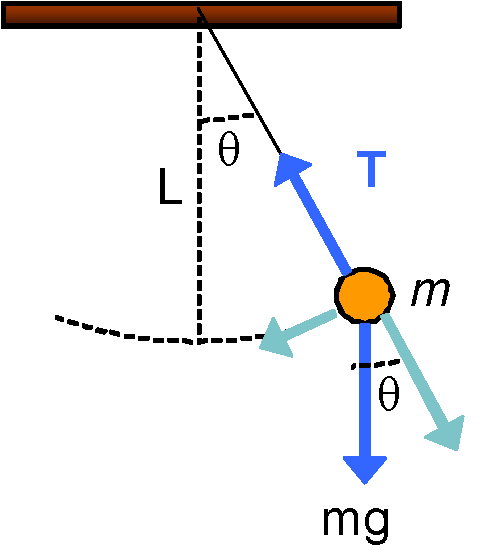
\includegraphics[width=0.5\textwidth]{Lab8_figs/simple_pendulum.pdf}

\end{center}

There are two forces acting on the pendulum bob: gravity, which pulls
downward, and the tension in the string. The acceleration of the bob can be
expressed in terms of a centripetal acceleration (parallel to the string)
and a tangential acceleration (perpendicular to the string). There is never
a change in velocity in the direction of the string, so the component of
gravity parallel with the string must equal the tension. The tangential
acceleration of the bob, which is what changes the bob's speed, is thus
provided by the component of gravity perpendicular to the string. If you do
the geometry, you find that this force has a magnitude of 
\[
F=-mg\sin \theta 
\]%
Putting this into Newton's second law, we end up with the relation 
\[
ma_{tan}=-mg\sin \theta 
\]%
The tangential acceleration is related to the angular acceleration by%
\sidenote{%
Understanding the details here is not so important as noticing that we are
again using Newton's second law to find the acceleration.} 
\[
a_{tan}=L\alpha 
\]%
where $L$ is the length of the string, and the angular acceleration ($\alpha 
$) is the second time derivative of the angular position, i.e. 
\[
\alpha =\frac{d^{2}\theta }{dt^{2}} 
\]%
Inserting these latter two expressions into our dynamic equation, we get 
\[
mL\frac{d^{2}\theta }{dt^{2}}=-mg\sin \theta 
\]%
At this point, the masses cancel and we can isolate the derivative on the
left hand side of the equation: 
\[
\frac{d^{2}\theta }{dt^{2}}=-\frac{g}{L}\sin \theta 
\]%
Despite it's relatively simple appearance, this second order nonlinear
ordinary differential equation does \emph{not} have a simple analytic
solution\sidenote{%
The analytic solution involves a few not-so-straightforward operations
involving differential calculus, as well as integrating the differential
equation twice. The second integration is an elliptical integral of the
first kind which generally can't be done without resorting to a numerical
method.}. At this point, most introductory physics texts use what is known
as a small angle approximation, i.e. for small angles $\sin \theta \approx
\theta $, where $\theta $ is in radians. Once that approximation is made,
the differential equation has exactly the same form as the equation for the
mass-spring system, and can be solved analytically. However, we recognize
that the solution will only be valid for small angles, generally less than
about $15^{\circ }$ (it is only really very good for very small angles $<%
\symbol{126}4\unit{%
%TCIMACRO{\U{b0}}%
%BeginExpansion
{{}^\circ}%
%EndExpansion
}$).

But what if you want to know something about the motion of the pendulum for
larger angles? You have two choices. Either you can go through the painful
process of solving the differential equation and numerically solving the
resulting integral (you physics majors will be able to do this by the time
you are seniors), or you can numerically approximate the solution to the
differential equation in a way that gives us useful information about how
the system behaves, even when the angles are large. In other words, you can
numerically model the pendulum. It is generally true that, with the
introduction of some intermediate variable (in our case $v$), that any
second order differential equation can be broken down into two coupled first
order ordinary differential equations. For the pendulum, these first order
equations are 
\begin{eqnarray*}
\frac{d\theta }{dt} &=&\omega \\
\frac{d\omega }{dt} &=&-\frac{g}{L}\sin \theta
\end{eqnarray*}%
This system (or any system like it) can be progressed forward in time using
Euler's method just as simply as the mass-spring system. Thus we can solve
any second order differential equation using Euler. For the pendulum, we can
find the motion without the pesky requirement that the angle be small. Where
no simple or easy analytic solution exists, we can still solve the system
numerically. This is a fantastic benefit that you physicists and engineers
will appreciate more as you take higher level classes!

It is worth noting that there are many more physical systems for which
analytic solutions simply cannot be found (not all differential equations
have analytic solutions). In those cases, you must solve numerically, there
is no other choice!\sidenote{%
You computer science majors have great job security!}

The easiest way to numerically model the dynamics of a system is to ask
three questions:

\begin{enumerate}
\item What is the current position or state of my system?

\item How fast is it moving, and in what direction?

\item Can I guess where the system will be a short time from now?
\end{enumerate}

This is just what we did in using Euler's method.







\end{document}